\chapter{Discussion}
\label{chap:discussion}
This chapter will discuss the main contributions of this thesis, namely the creation of the TinyFuncData dataset in section \ref{sec:datadisc} and the training of the TinyFuncCoder series in section \ref{sec:trainingdisc}.
It will also discuss the evaluation of the TinyFuncCoder models in section \ref{sec:evaldisc} and what research could build on these results in the future in section \ref{sec:future}.

\section{Dataset Creation}
\label{sec:datadisc}
This section will discuss the creation of the TinyFuncData dataset, the assumptions and decisions that were made in its creation and the problems that may have occured.
The dataset was intended to be a gathering of high-quality function definitions in common programming languages that include a natural language description in the form of a docstring.
The decisions to limit the dataset to the top ten languages of GitHub was made to ensure that only the most relevant languages that a student might interact with are trained on.
However, there is still a massive discrepancy in the amount of training data per language, with Python being over half of the data, and TypeScript not even contributing half of a percent.
A model that focuses only on a single language or fewer languages may be less confused by the varied syntax in multiple programming languages, and a hypothetical use in a classroom setting could be limited to a single programming language.
Feng et al. find that training single-language models proved to be more effective than multi-language models in their paper introducing CodeBERT \cite{Feng.19.02.2020}.
The most obvious choice here is Python, which has the majority of the data and is the most widely used in the field of \acp{lm}.
On the other hand, Wei et al. assert that learning on multiple languages can provide a deeper understanding of the code, with concepts only trained in one language being applied when prompted in another in the paper introducing Magicoder \cite{Wei.2024}.
TinyFuncData is also doubly bilingual.
Because data is taken from The Stack, a large gathering of GitHub data, many of the files contain docstrings in languages other than English.
English is the preferred language, as most \acp{lm} are trained either in English or Chinese, and the target user group is much more likely to be familiar with the former.
Having docstrings in other languages and with other alphabets than the one(s) the model is trained on could also weaken the correlation between the docstring and its code.
To remedy this, one could either filter out all non-English docstrings or translate all text into English, but both approaches come with their own downsides.
Excluding multilingual data entirely removes code content for the model to learn.
Translating all docstrings would have to be done automatically.
This is risky, as docstrings often also contain deliberate word choices, names of variables and sometimes even ASCII-art or basic separations of text through long lines of symbols, all of which could easily be translated incorrectly by an automatic process.

Next, three decisions were made when creating the \ac{regex} for data filtering.
First, imports were not included.
Imports are typically grouped at the top of a code file, with no easy way to discern which import is used in which function.
Adding a filter for which imports belong to which functions would have vastly increased the complexity of the \ac{regex} if it is possible at all.
Another option would have been to include all imports of a file with the function definition of every function of that file.
This was decided against to prevent the model from randomly including imports that are unnecessary, but it may have come at the cost of valuable information about the functions.

Second, TinyFuncCoder was intended to generate code from function descriptions while requiring the user to pre-plan an architectural context in which that function is used.
However, there is currently no intended way to tell the model which functions already exist to be called within the current function, which goes against this planning.
Using only isolated functions that do not interact is not realistic in practice.
Gathering data for which calls a function makes in its body would have also complicated dataset creation, and also created another issue.
The model should ideally know what the function that is being called can do, and thus would ideally also have a docstring to read.
Adding so much information could add a lot of extra context for the model to parse, clouding the important information with bloat.
Taking this to the extreme, there would be a wide recursion of function information for all sub-sub-sub-calls of a function.
On the other hand, providing only the called function names and perhaps parameters assumes that they are named in a self-explanatory manner, which is an optimistic assumption.

Third, and with the most direct impact on the dataset, is the decision to only consider docstrings that are given \emph{before} the function head.
During the filtering from TinyFuncData-dedup to TinyFuncData-docstring, all data points with an empty docstring column are deleted.
As the \ac{regex} only matches docstrings before the head, this deletes all functions where it lies within the body.
This is done because it is practically impossible to differentiate a first-line comment from a proper docstring if it is in the body, but it presumably excludes additional data that could have been used in training.
However, this also directly leads into problems with the evaluation, as many of the metrics format their data to have the problem description docstring after the function head.
Since TinyFuncCoder's prompt template has all training data formatted with docstrings before the function, it is reasonable to assume that the problems should be reformatted to fit TinyFuncCoder's expected data scheme.
The evaluation presented in chapter \ref{chap:results} backs this up, with TinyFuncCoder-v1.0 often performing better when the prompt is reformatted.
This may also explain why some the amount of data for some languages drops steeply and unexpectedly during the filtering from TinyFuncData-dedup to TinyFuncData-docstring.

All of these decisions can be changed without having to recreate the dataset from scratch, but would still require heavy time investment.
As the dataset still includes the id of the original file from which they were collected, a secondary run through the data could be done to collect the imports, including them as a new column in the dataset.
However, this would require another pass through most of The Stack dataset.
Function calls in a function can still be gathered through a new \ac{regex} written for this purpose applied to the body column of any of the dataset versions.
Functions with interior docstrings can be gathered from TinyFuncData-dedup, before the docstring filter is applied.
The \ac{regex} only matches the docstring before the function head optionally, so functions where it comes after should still be included in the data.
This would also require a new \ac{regex}.

Finally, an error was discovered in the dataset creation process after the training of the TinyFuncCoder models was already concluded.
The docstring group of the \ac{regex} for filtering functions only matched the last comment line when using multiple single-line comments (\enquote{// \dots$\backslash$n//\dots}) rather than a multiline comment (\enquote{/** \dots */}).
This was not discovered earlier despite sampling data because all of the sampled data included docstrings that were already only one line long.
A new version of the dataset creation script has been created to address this issue which is provided in the repository.
However, attempting to run this new script took much, much longer than the original.
The new script was run for 24 hours to collect the data for Java and it only covered 1.521 rows of The Stack and extracted 336 \enquote{proper} function definitions.
This data is available on huggingface\footnote{\url{https://huggingface.co/datasets/JanDkff/TinyFuncData-Java} (last visited on 2024-11-04)}.
Of these, 297 begin with \enquote{/**}, meaning they use a multiline comment.
Only 39 begin with \enquote{//}, which is the part of the \ac{regex} that is incorrect, around 13\% for this small sample.
Python is unaffected by this, as it was parsed using the \texttt{ast} library, not with a \ac{regex}.
While this thesis is unaware for similar Python libraries for the other programming languages, an alternative to the time-consuming \ac{regex} gathering process would be implementing new \ac{ast} libraries in Python.

With over half of the data being Python, the effects of this might be limited.
Had this been noticed during the original dataset creation, TinyFuncCoder would have been trained only on Python data.
For future work, a dataset containing only the Python data was created and made available on huggingface\footnote{\url{https://huggingface.co/datasets/JanDkff/TinyFuncData-Python} (last viewed on 2024-11-04)} alongside the other versions.


\section{Training}
\label{sec:trainingdisc}
This section will discuss the training of the TinyFuncCoder series, and how the decisions made during training could have led to the subpar model performance, especially for v1.1, which except for a single correct answer on MBPP+ scores a pass@1 of zero on all metrics.
All decisions made during training were made with the intent to make training viable with the given hardware, most critically with respect to memory.
Memory crashes were a constant issue throughout training, and many tradeoffs were made because of this.
As such, parameters were often set to very low values which likely impacted the models ability to learn.
One big issue directly caused by the memory crashes, which was already mentioned in section \ref{sec:loss}, is that crashes forced a restart of the training process from checkpoints, which presumably lead to the reset of the trainer and optimizer states, which likely effected the training process.
It is also possible that the custom code swapping out the dataset for each epoch of training effects the training process.
Another limiting factor might be creating a model that generates purely left-to-right, despite code being structured and written differently than natural language.

TinyLlama was chosen as the base model as it is a decently small model with some code knowledge, but not much.
For training TinyFuncCoder, it was deemed preferrable that only a moderate amount of code training is present to prevent the model from generating code that goes beyond the extents of its intended purpose -- a single function, written from the constraints of the input.
After TinyFuncCoder-v1.0 did not improve much on TinyLlama-v1.0, TinyLlama-v1.1 was used to test if the fine-tuning process made enough of a difference to teach the model any code knowledge, which it did not.
This is probably caused by the many tradeoffs made to be able to fine-tune this model at all, which begs the question if it was indeed the best choice as a base.
Perhaps choosing an even smaller model or fine-tuning a model purely from scratch would have yielded better results.
For comparison, the 350 M parameter CodeGen model achieves a pass@1 of 12.76 on HumanEval \cite{Nijkamp.2022}, the same as TinyLlama-v1.0.

After training concluded, some experimental training was done to see if a more promising approach could be found for future work.
One test used a more radical prompt that included tags for the programming language, docstring, function head and function body, though this quickly resulted in a model that only generated tags.
Fine-tuning Phi-1, the smallest Phi model, instead of TinyLlama did not change its performance much either, and neither did testing done with the supervised fine-tuning trainer class SFTTrainer\footnote{\url{https://huggingface.co/docs/trl/v0.12.0/sft_trainer} (last visited on 2024-10-31)} from huggingface.
All of these experiments were only a few epochs long.

Another possible point of contention is the amount of data the model is fine-tuned on.
The data that v1.0 saw during training encompasses around 1 B tokens -- 1,024 tokens per function, with 25 chunks of the dataset, with 80\% of a chunk being used for training and 6,401,534 rows in total; $6,401,534 \cdot 0.25 \cdot 0.8 \cdot 1,024 = 1,311,034,160$.
In comparison, most of the \acp{lm} discussed in sections \ref{sec:basemodels} and \ref{sec:synthmodels} were trained on over a trillion tokens.
The amount of data used in training may simply not be enough to tune the model enough for its intended task, especially if it is limited by the other concessions being made during training.
Further, TinyLlama was trained on Starcoderdata -- a derivative of The Stack.
TinyFuncData is also derived from The Stack.
While further fine-tuning on data that has already been seen by a model is not necessarily pointless, it could result in a smaller improvement than if presented with new code data.
Overall, while it is very hard to conclusively determine the cause of the suboptimal training performance, it is likely a combination of the above mentioned points.
Under the given time and hardware constraints, an extensive hyperparameter analysis and more tests with different models were not possible.
It may also simply be the case that the combination of all restraints make fine-tuning a model of the desired capabilities near impossible.

\section{Evaluation}
\label{sec:evaldisc}
This section will discuss the evaluation process of the TinyFuncCoder models and the TinyLlama models, as both were evaluated with the same metrics and through the same generation and evaluation pipeline.
The chosen metrics contain the most popular metrics currently in use to evaluate code synthesis models and also use lesser-known metrics to more fully judge the models capabilities.
All suitable metrics from the Bigcode Evaluation Harness, as well as the additional Leetcode Contest Benchmark were chosen.
Most of the code from the Bigcode Evaluation Harness could be used for evaluating most metrics, with minor adjustments, but DS-1000 and the Leetcode Contest Benchmark required more heavily altered and custom-written implementations.

One of the weakpoints of the chosen metrics is their diversity.
HumanEval(+), MBPP(+), DS-1000 and the Leetcode Contest Benchmark all only pose problems in Python.
The other two metrics, MultiPL-E and HumanEvalPack only translate the original HumanEval problems into other languages, but do not pose their own problems which may be better suited or even aiming at unique features of a language.
This is a large bias towards a single programming language that even leaves C, the second largest language of the dataset, completely untested.
Interestingly, this heavy bias towards Python is also reflected in the training data, where over half of all function definitions come from Python.
This bias towards Python is likely caused by its prominence as a language in the \ac{nlp} field.
As posited in chapter \ref{sec:data}, it may be the case that a sizeable chunk of the Python data used in the TinyFuncData dataset could also be \ac{lm}-generated, raising concerns over the quality of the data and creating an \ac{ai} feedback loop.
An indicator of this could be Python data with a single-line docstring, as code synthesis \acp{lm} only rarely generate multiline comments, but this is hard to definitively prove.
For Python, 1.65 M of 3.41 M rows have a docstring of just one line, or about 48\%.

\begin{comment}
The entire distribution of docstring line counts and length is shown in figure \ref{fig:docdist}.
\begin{figure}[h]
    \centering
    \begin{minipage}{0.5\textwidth}
        \centering
        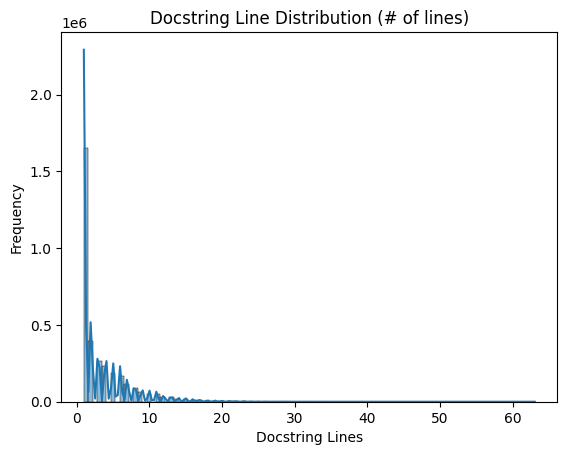
\includegraphics[width=\textwidth]{kapitel6/docline.png}
    \end{minipage}\hfill
    \begin{minipage}{0.5\textwidth}
        \centering
        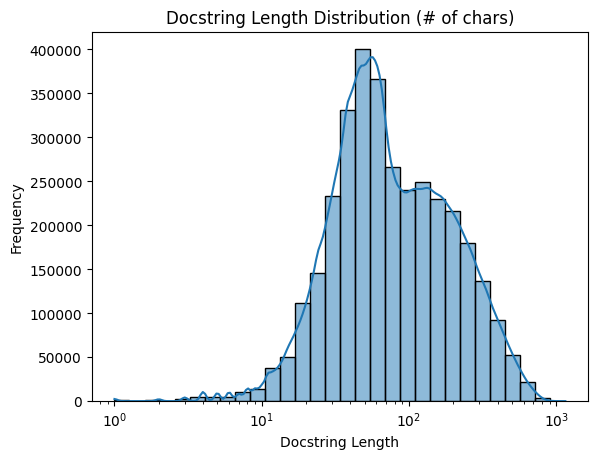
\includegraphics[width=\textwidth]{kapitel6/doclen.png}
    \end{minipage}
    \caption{Distribution of the number of docstring lines and docstring length in TinyFuncData-Python.}
    \label{fig:docdist}
\end{figure}
\end{comment}

Some of the metrics also are likely not reliable indicators of model performance.
The most concerning are MultiPL-Es PHP and Go evaluations, which produce suspiciously good results and cause occasional crashes, all of HumanEvalPack, which produced pass@1 values of zero on languages which had already provided better results on MultiPL-E, and the Leetcode Contest Benchmark, which could not be evaluated due to the lack of a proper Docker environment.
DS-1000 also provides suspiciously poor results, but this could be accurate when compared to the performance of other models.
Also, the creation of HumanEval, the basis for many of the other metrics and perhaps the most well used, is only barely mentioned in the paper where it was introduced, with a longer description in the appendix that also does not specify much about the creation process and mostly goes into detail about the properties that an evaluation set should have.

\section{Future Work}
\label{sec:future}
There is no shortage of research being done in the code synthesis \ac{llm} field, with many new advancements being made while this thesis was being written.
However, no model that this thesis is aware of fulfills the specific purpose outlined within the section \ref{sec:motivation}.
To reiterate, the research question is \emph{How well can a small \acl{lm} be fine-tuned to only synthesise function bodies from a function signature using limited hardware?}
Because no model fulfills TinyFuncCoder's use case, further research into this field is desirable to improve upon the first attempt made by the TinyFuncCoder models.

For further research, the following should be attempted or kept in mind:
TinyFuncData-Python is a solid baseline to work off of.
The evaluation metrics used, while not perfect, provide solid insight into the capabilities of a model and can be used in the future if the obsolete and non-functioning metrics are removed.
More experimentation with data structuring for training should be done.
A simple suggestion is to approach training as a natural language to code task, where the natural language docstring is seen as the input and the entire function as the output.
This was not attempted for TinyFuncCoder because the head was considered part of the input, something that the user should be able to define, but more strictly segmenting between code and language could be useful.
TinyLlama should be reevaluated as a base model, considering it did not improve much with fine-tuning on most metrics and is worse than comparable models of its size, though this could also be seen as a benefit.
While training a model from scratch might be a good solution, that prevents the use of the \ac{peft} techniques that made training possible at all.
A freshly trained model would have to be much smaller than the current 1.1 B parameters or require better hardware and more training time, and would also lack preexisting natural language and possibly code knowledge.
A good approach to try could be the recently-released \ac{qdora} \cite{Liu.2024b}, a merging of the quantization approach of \ac{qlora} and the improvements \ac{dora} \cite{Liu.2024b} makes to \ac{lora} that claims to be as resource-efficient as \ac{qlora} while improving performance to be close to full fine-tuning \cite{Liu.2024b}.
Finally, the best \ac{lm} of 1.5 B and fewer parameters that this thesis is aware of, DeepSeekCoder-1.3B-Base, achieves a pass@1 of 30\% on HumanEval.
Model size seems to be correlated to performance on this metric.
Any potential near-future work to create a TinyFuncCoder model trained from a small \ac{lm} will most likely also achieve a pass@1 of 30\% at best, making it unreliable as a coding assistant even in the best case scenario.
This is especially problematic in its intended setting, a classroom, where a less experienced student may not easily spot or understand mistakes made by the model.